\documentclass[12pt]{article}
\usepackage[utf8]{inputenc}
\usepackage{amsmath,amssymb}
\usepackage{unicode-math}
\usepackage[T2A]{fontenc}
\usepackage[russian]{babel}
\usepackage{graphicx}
\usepackage{subfigure}
\usepackage{subcaption}
\usepackage{url}
\usepackage{float}


\DeclareGraphicsExtensions{.pdf,.png,.jpg}
\usepackage{hyperref}
\usepackage{wrapfig}
\usepackage[left=20mm, top=20mm, right=10mm, bottom=20mm]{geometry}

\usepackage{amsmath} 
\usepackage{amsfonts} 
\usepackage{amssymb} 
\usepackage{wasysym} 
\usepackage{fancyhdr}

\pagestyle{fancy}
\fancyhf{}
\lhead{Семинар 7. Спин. Сложные атомы}
\rhead{\textit{Клименок К.Л., МФТИ 2020}}
\rfoot{\thepage}



\begin{document} 
\title{\textbf{Семинар 7. Магнитный момент. Спин. Сложные атомы}}
\author{\textbf{Клименок Кирилл Леонидович}}
\date{18.09.2020}
\maketitle
\section{Теоретическая часть}

\subsection{Связь магнитного и орбитального момента}
Перед тем, как вводить понятие спина, надо начать со связи магнитного и механического моментов. Для это рассмотрим классическое представление об электроне, как о заряженном шарике вращающемся вокруг ядра. 
\begin{figure}[h]
    \centering
    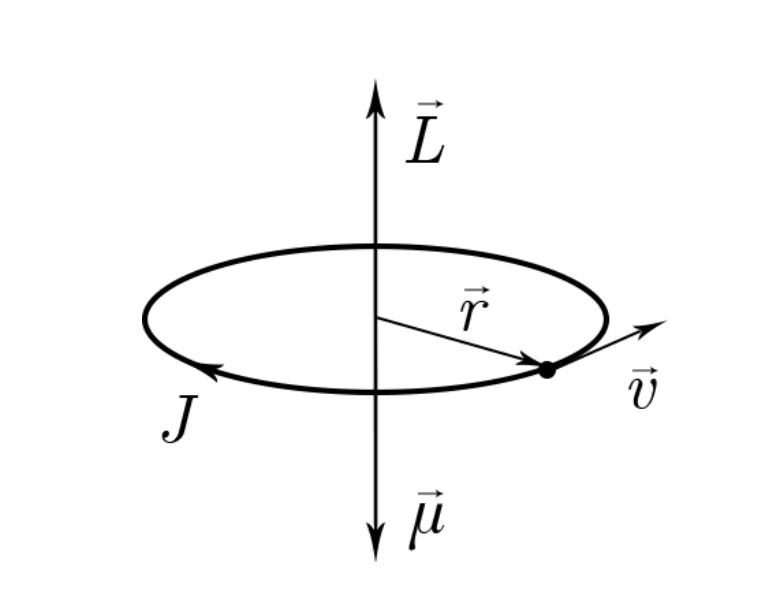
\includegraphics[width=0.5\textwidth,height=\textheight,keepaspectratio]{Seminar_07/pics/pic_01.PNG}
    \caption{Демонстрация связи механического и магнитного моментов в классической модели для электрона в атоме. $J$ -- сила тока, $\mu$ -- магнитный момент}
    \label{fig:sem_7_gymagnetic_ratio}
\end{figure}
Мы можем записать механический и магнитный моменты для такого электрона:
\begin{gather*}
    \textbf{L} = [\textbf{r} \times m\textbf{v}] = rmv \textbf{n}\\
    \mu = \dfrac{J\textbf{S}}{c} = \dfrac{1}{c} \dfrac{ev}{2\pi r}\pi r^2 \textbf{n} = - \dfrac{e}{2c} rv\textbf{n} \dfrac{m}{m} = -\dfrac{e}{2mc}\textbf{L}
\end{gather*}
Видно, что в рамках такой классической модели есть четкая связь механического и магнитного моментов. Скорее всего и в квантовом мире эта связь должна сохраниться, а поскольку проекция момента импульсам на выбранную ось квантуется $L_z = m_z \hbar, m_z = \0, \pm 1, \dots, \pm l$, $l$ -- максимальное значение орбитального момента, то, получается, что и проекция магнитного момента должна квантоваться. Единственное, что дополнительно должно появиться -- это какой-то не очевидный коэффициент, который мы будем обозначать $g$ и называть далее g-фактором или фактором Ланде:
\begin{equation}
\mu = -g\cdot \dfrac{e\hbar}{2mc} m_z = -g \mu_{\text{Б}} m_z   
\end{equation}
$\mu_{\text{Б}} = 927 \cdot 10^{-26} \frac{\text{Дж}}{\text{Тл}} = 0.927 \cdot 10^{-20} \frac{\text{эрг}}{\text{Гс}}$ -- магнетон Бора
\subsection{Экспериментальное подтверждение связи магнитного и орбитального момента. Спин.}
Понятно, что теорию мы можем написать какую угодно, но мы на общей физике, поэтому надо бы как-то проверить, что описанное выше имеет смысл. Поэтому рассмотрим 2 эксперимента, которые действительно подтверждают ее.
\paragraph{Опыт Эйнштейна и да Гааза}
Опыт предельно прост по своей сути -- мы помещаем цилиндр из ферромагнетика во внешнее поле и подвешиваем его на нитке. Далее резко изменим магнитное поле на противоположенное. Тогда,все магнитные моменты атомом поменяют ориентацию, что повлечет за собой изменение момента импульса и наш цилиндр начнет вращаться. Оценить этот эффект можно, если приравнять приобретенный момент импульса всего тела ($I\omega$) к моментам импульса всех электронов в нем ($N\cdot 2L_{e}$). Из характерных оценок для цилиндра массой 100 грамм и радиусом 1 см, характерная угловая скорость получается около $10^{-3}$ Гц, что довольно сложно детектировать. В оригинальном опыте исследовали не полученную угловую скорость, а крутильные колебания. Сначала получали все параметры колебательной системы без внешнего поля, а потом измеряли амплитудно-частотную характеристику, в зависимости от частоты перемагничивания. По полученной кривой и был найдена связь магнитного и механического момента, а g-фактор для электрона оказался равен 2 с хорошей степенью точности
\footnote{Примечание: вообще-то о g-факторе изначально не говорили и реальный результат примерно соответствовал соотношению $\mu = - \mu_{\text{Б}} m_z$, что было связано с ошибками в эксперименте, только дальнейшие более точные эксперименты открыли реальное положение дел.}
\paragraph{Опыт Штерна-Герлаха}
Суть опыта также предельно проста. У нас есть источник нейтральный атомов серебра, у которых на внешней орбитали 1 электрон (это позволяет говорить, что это водородоподобный атом). Пучок этих атомов проходит через специальный магнит с сильно неоднородным магнитным полем. Так как в неоднородном поле на магнитный диполь действует сила (привет 3 семестру), то такой атом должен отклониться от своей траектории (при этом это не сила Лоренца -- атом нейтрален). В классическом случае, если бы механический, а значит и магнитный, моменты атома были непрерывны, то на экране мы бы видели четкую полосу в зоне попадания атомов. Однако, еще в прошлом семинаре мы видели как механический момент электрона в атоме квантуется и может иметь различное значение проекций на выделенную ось. Одна проблема -- проекций всегда нечетное число, а в эксперименте явно наблюдается расщепление на 2 точки. Это может означать только одно -- у электрона есть собственный магнитный момент, который мы будем называть спином. Он также квантуется и может принимать значения $\pm \dfrac{1}{2}\hbar$. Это является следствием более ранней договоренности считать расщепление как $2S+1=2$. 
\begin{figure}[h]
    \centering
    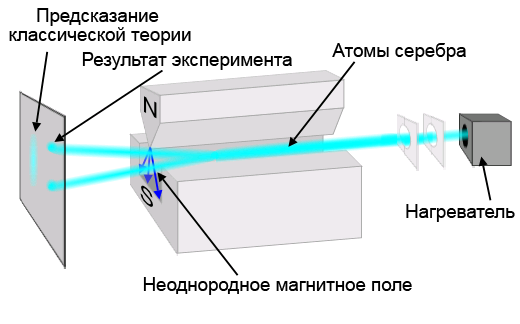
\includegraphics[width=0.5\textwidth,height=\textheight,keepaspectratio]{Seminar_07/pics/pic_02.png}
    \caption{Установка для опыта Штерна-Герлаха}
    \label{fig:sem_7_gymagnetic_ratio}
\end{figure}
\paragraph{Спин} Подводя итоги по этим 2 экспериментам мы видим, что у электрона в атоме появился собственный магнитный момент -- спин, который не имеет классической аналогии и квантуется как $\pm \dfrac{1}{2}\hbar$. При этом мы в рамках нашего курса просто его постулируем. Более честный вывод наличия спина представлен в релятивистской квантовой теории на теорфизике. 
И вот теперь мы можем полностью описать состояние электрона в атоме. Для этого нам нужно 4 квантовых числа, а именно $n$ -- главное квантовое число (описывает уровень энергии), $l$ -- орбитальное квантовое число (момент импульса), $m$ -- магнитное (проекция момента импульса на выделенную ось), $s$ -- спиновое (какую проекцию имеет спин). И теперь имеет смысл комментарий к таблице из 6 семинара о степенях вырождения уровней энергии как $2n^2$. На самом деле это очень хорошо видно в таблице Менделеева. В первом периоде только 2 элемента: водород и гелий, заполнено состояние с $\{n = 1; l=0; m=0; s=\pm1/2\}$. Во втором периоде 8 элементов с состояниями с $\{n = 2; l=0,1; m=0,\pm1; s=\pm1/2\}$ и так далее. 
\subsection{Сложение моментов. Полный момент атома.}
Естественным продолжением разговора о моментах является разговор об их сумме, так как атом это замкнутая система и при взаимодействии с внешним полем у нас получается, что надо рассматривать и орбитальный и спиновый моменты электронов. \\
Начнем с простого: пусть у нас есть 2 момента $L_1, L_2$ и мы хотим их сложить. Поскольку мы работаем с квантовой механикой, то нам надо перейти к их операторам и решить задачку на собственные числа суммарного оператора. Но естественно честно я решать это не буду, а просто вспомню, что у нас моменты квантуются и максимальные значения проекций на выбранную ось для этих операторов будут $l_1, l_2; l_1>l_2$ соответственно. Тогда максимально возможная проекция момента будет их суммой $l_1 + l_2$, когда их направления совпадают, а минимально возможная проекция равна их разности $l_1 - l_2$, когда они направлены в разные стороны. при этом все значения между ними также возможны. Тогда количество всевозможных состояний для этих моментов:
\begin{equation*}
    N_{tot} = \sum\limits_{l=l_1-l_2}^{l_1+l_2}2l+1 = (2l_1+1)(2l_2+1)
\end{equation*}
Теперь давайте разберемся с более сложной вещью, а именно с суммированием полного магнитного момента. Для определенности будем рассматривать электрон с орбитальным моментом $L$ и спиновым моментом $S$. Для них магнитные моменты:
\begin{gather*}
    \mu_l = -g_l\mu_{\text{Б}}l\\
    \mu_s = -g_s\mu_{\text{Б}}s\\
\end{gather*}
при это вообще-то у них разные факторы Ланде. введем полный момент импульса $J = L+S$, и для сохранения единообразия запишем полный момент аналогично: 
\begin{gather*}
    \mu_j = -g_j\mu_{\text{Б}}j\\
\end{gather*}
Строго выводить формулу для g-фактора в этом случае я не буду, просто ограничусь тем, что скажу, что полный магнитный момент не сонаправлен с полным механическим моментом и из геометрии его проекцию на $\textbf{J}$ вполне можно получить. Сам ответ для суммарного g-фактора:
\begin{equation*}
    g_j = 1+\dfrac{J(J+1) + S(S+1) - L(L+1)}{2J(J+1)} 
\end{equation*}
\paragraph{Терм}
Вот теперь, когда мы ввели все квантовые числа для атома и даже научились складывать моменты можно поговорить о том, как в физике принято записывать состояния атома. Но для начала вспомним, что мы делали в рамках школьной химии и поймем почему нам это не подходит. Там мы заполняли все орбитали последовательно, так что в результате получали полную электронную конфигурация всех электронов. Например для атома натрия электронная конфигурация $1s^22s^22p^63s^1$. Она дает представление общем количестве электронов и о том, что последний электрон расположен на орбитали $3S$ участвует в валентных связях, но не дает представление об орбитальном, спиновом и полном моментах атома, а ведь именно расщепления по ним и наблюдают в физических экспериментах. Здесь нам на помощь приходит другая форма записи, а именно терм. Ее общий вид:
\begin{equation*}
    n^{2S+1}L_J
\end{equation*}
Здесь обозначения совпадают с введенными нами ранее. Единственное, что $L$ обозначается буквой в соответствии с таблицей:
\begin{table}[H]
\begin{tabular}{|l|l|l|l|l|l|}
\hline
\multicolumn{1}{|c|}{} & \multicolumn{1}{c|}{S} & \multicolumn{1}{c|}{P} & \multicolumn{1}{c|}{D} & \multicolumn{1}{c|}{F} & \multicolumn{1}{c|}{G} \\ \hline
L                      & 0                      & 1                      & 2                      & 3                      & 4                      \\ \hline
\end{tabular}
\end{table}
При этом в наших задачах может отсутствовать какая-то из частей записи терма, которая не нужна в решении.
\paragraph{Заполнение орбиталей. Принцип запрета Паули и правила Хунда.}
Теперь мы научились записывать состояния электронов в сложном атоме, но как их надо заполнять? Понятно, что основное состояние будет с минимальной энергией, но как это определить? Тут работает 2 базовых правила. \\
\textit{Принцип запрета Паули.} Электроны, как частицы с полуцелым спином, фермионы, не могут существовать в одном энергетическом состоянии со всеми одинаковыми квантовыми числами. Это означает, что даже если у 2 электронов в атоме одинаковые n, l и m, то проекции спина у них должны быть направлены в разные стороны.\\
\textit{Правила Хунда.} Это эмпирический набор правил заполнения энергетических оболочек атомов, схожий с тем, что было в школьной химии. Ниже по энергии лежит тот атомный терм, для которого выполняются два условия:
\begin{enumerate}
    \item Мультиплетность ($2S+1$) максимальна
    \item При совпадении мультиплетностей суммарный орбитальный момент $L$ максимален
\end{enumerate}



\subsection{Тонкое и сверхтонкое расщепление}
Перед тем как двигаться к задачам нужно упомянуть еще о паре вещей, а именно о расщеплении уровней энергии из-за всей вот этой нагороженной выше теории. Я не буду сильно грузить вас этим, а попробую рассказать это максимально понятно из имеющегося у вас опыта. 
\paragraph{Тонкое расщепление. LS-связь}
Чтобы понять, что происходит, нам поможет классическое представление. Конечно это не комильфо, но так реально понятнее. Вернемся к нашей самой первой модели из этого семинара и сядем на электрон. Он неподвижен и имеет магнитный момент, заряженное ядро вращается вокруг него и создает внешнее поле, в котором магнитный момент будет ориентироваться по или против поля, тем самым меняя свою энергию. Это и есть тонкое расщепление. Если же мы будем рассматривать это со стороны стороннего наблюдателя, то получится что-то типа барона Мюнхгаузен, вытягивающего себя за волосы из болота. То есть электрон летает по орбите и взаимодействует сам с собой. Вот именно поэтому классическое представление понятнее.\\
Оценим, от чего зависит энергия этого расщепления. Тут все очень просто -- от орбитального момента зависит то как вращается вокруг нас ядро и соответственно внешнее поле, а также от спина электрона. Итого получаем: 
\begin{equation*}
    \Delta U_{LS} \sim (\mu_S B_L) \sim  ( \hat{L}\hat{S} )
\end{equation*}
Осталось научится оценивать такие скалярные произведения. Для этого воспользуемся следующим выводом:
\begin{gather*}
    \hat{J}=\hat{S}+\hat{L}\\
    \hat{J^2}=\hat{S^2}+\hat{L^2} + 2 (\hat{L}\hat{S})\\
    (\hat{L}\hat{S}) = \dfrac{1}{2} \left(\hat{J^2} -\hat{S^2} -\hat{L^2} \right) = \dfrac{1}{2} \left(J(J+1) -S(S+1) -L(L+1) \right)
\end{gather*}

\paragraph{Сверхтонкое расщепление.}
Тут все существенно проще. У ядра тоже может быть спин, который создает магнитное поле вокруг себя, которое в свою очередь будет взаимодействовать со спином электрона.


\section{Практическая часть}
\subsection{Задача 6.9}
\label{task_6.9}
\paragraph{Условие}
С какой угловой скоростью $\omega$ и в каком направлении должен начать вращаться цилиндр, подвешенный магнитном поле $B$, направленном параллельно его оси вертикально вверх, если изменить направление поля на обратное? Считать, что цилиндр намагничивается до насыщения. Момент импульса электрона в атоме равен $k$, число атомов в
цилиндре $N$, момент инерции цилиндра $I$.
\paragraph{Решение}
Тут как и в теоретической части нужно приравнять момент импульса цилиндра как целого и момент импульса каждого отдельного атома:
\begin{equation*}
    I\omega = 2kN \Rightarrow \omega = \dfrac{2kN}{I}
\end{equation*}

\subsection{Задача 6.15}
\label{task_6.15}
\paragraph{Условие}
Параллельный пучок нейтронов с энергией $T = 0.025$ эВ проходит через коллимирующую щель шириной $ d= 0.1$ мм и затем через зазор в магните Штерна–Герлаха длиной $L = 1$ м. Оценить значение градиента поля $\frac{dB}{dz}$, при котором угол магнитного отклонения компонент пучка равен углу дифракционного уширения. Магнитный момент нейтрона $\mu_n = 9.66 \cdot 10^{−24}$ эрг/Гс.
\paragraph{Решение}
У нас тут 2 процесса, которые отклоняют наш пучок нейтронов. Первый -- дифракционное уширения на щели, так как нейтроны все-таки квантовые частицы. Второй -- отклонение в неоднородном магнитном поле за счет спина. вопрос откуда он там взялся у нейтральной частицы оставим за границами этой задачи. При этом первый процесс может пересилить второй, и тогда вместо расщепления мы увидим сплошную полосу. 
\begin{figure}[h]
    \centering
    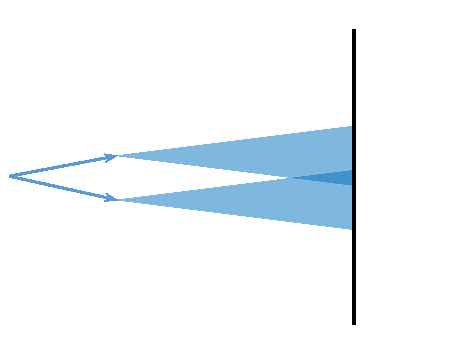
\includegraphics[width=0.5\textwidth,height=\textheight,keepaspectratio]{Seminar_07/pics/pic_03.pdf}
    \caption{Расщепление почка нейтронов в задаче 6.15 }
    \label{fig:sem_04}
\end{figure}
Оценим дифракционное уширение:
\begin{equation*}
    \alpha_{\text{диф}}= \dfrac{\lambda}{d} = \dfrac{h}{d\sqrt{2mT}}
\end{equation*}
Рассчитаем отклонение под действием силы со стороны магнитного поля. Для этого разделим скорость на 2 компоненты продольную $v_{\parallel}$ и поперечную $v_{\perp}$ и свяжем их между собой. По сути это кинематическая задачка:
\begin{gather*}
    f_{\perp} =m a_{\perp} = \mu_n \dfrac{dB}{dz}; \Rightarrow a_{\perp} = \dfrac{\mu_n}{m} \dfrac{dB}{dz}\\
    v_{\perp} = a_{\perp} \tau, L=v_{\parallel}\tau; \Rightarrow v_{\perp} = \dfrac{\mu_n}{m} \dfrac{dB}{dz} \dfrac{L}{v_{\parallel}}\\
    \alpha_{\text{маг}}= \dfrac{v_{\perp}}{v_{\parallel}} = \dfrac{\mu_n \dfrac{dB}{dz} L}{mv^2_{\parallel}} \approx \dfrac{\mu_n \dfrac{dB}{dz} L}{2T}
\end{gather*}
По условию приравниваем углы отклонения между собой и получаем:
\begin{equation*}
    \dfrac{dB}{dz} = \dfrac{2Th}{L\mu_nd\sqrt{2mT}} \approx 150 \dfrac{\text{Гс}}{\text{см}}
\end{equation*}

\subsection{Задача 6.76}
\label{task_6.76}
\paragraph{Условие}
В спектрах газовых туманностей наблюдаются линии, которые долгое время не могли приписать ни одному из известных элементов. В последствии выяснилось, что это линии ионов кислорода и азота. Наиболее интенсивные линии соответствую переходам $^1D_2 \rightarrow ^3P_2$, $\lambda_1 = 5007$ \AA\text{ } и $^1D_2 \rightarrow ^3P_1$, $\lambda_2 = 4959$ \AA\text{ }для иона кислорода $O^{++}$. Найти длину перехода $^3P_1 \rightarrow ^3P_0$ с использованием схемы Рассела-Саундерса (LS-схема).\\
\textit{Указание}. В этой схеме энергия спин-орбитального взаимодействия равна $A( \hat{L}\hat{S} )$
\paragraph{Решение}
Задача выглядит максимально сложно, но все-таки давайте ее раскрутим. Для того чтобы понять ее для такого иона нарисуем все возможные термы и посмотрим, что за переходы между ними нам даны и что от нас хотят найти. Для того, чтобы понять какие термы возможны нужно во-первых записать все возможные значения проекции момента импульса для 2 электронов на 2p-орбитали ($\pm 2, \pm 1, 0$) и все возможные значения проекций суммарного спина ($\pm 1, 0$). Во-вторых, воспользоваться правилами запрета Паули и правилами Хунда. В результате перебора всех вариантов получится 15 всевозможных комбинаций, который по энергиям представлены на рисунке. 
\begin{figure}[h]
    \centering
    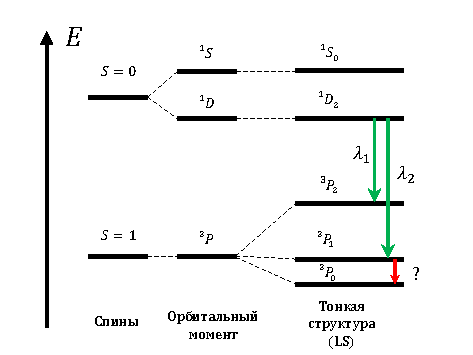
\includegraphics[width=\textwidth,height=\textheight,keepaspectratio]{Seminar_07/pics/pic_04.pdf}
    \caption{Структура уровней энергии для задачи 6.76}
    \label{fig:sem_04}
\end{figure}
Также из него сразу видно, что нам дано,  а именно длины волн (по сути разность энергий) для 2 зеленых стрелочек, и надо найти разность энергий для красной стрелки. При этом тонкая структура терма $^3P$ определяется как раз таки известной нам формулой (схема Рассела-Саундерса).
\begin{equation*}
    E_{LS} = A(\hat{L}\hat{S} ) = \dfrac{A}{2}\left(J(J+1) - S(S+1) -L(L+1) \right)
\end{equation*}
Давайте с ее помощью запишем разность энергий этих уровней:
\begin{gather*}
    E(^3P_2) - E(^3P_1) = [E(^3P)+E_{LS}(J=2)] - [E(^3P)+E_{LS}(J=1)] = \dfrac{A}{2}(2\cdot 3 - 1\cdot2)= 2A\\
    E(^3P_1) - E(^3P_0) = [E(^3P)+E_{LS}(J=1)] - [E(^3P)+E_{LS}(J=0)] = A\\
\end{gather*}
Теперь реализуем данные о переходах из условия:
\begin{gather*}
\begin{cases}
    E(^1D_2) - E(^3P_2) = \dfrac{hc}{\lambda_1}\\
    E(^1D_2) - E(^3P_1) = \dfrac{hc}{\lambda_2}
\end{cases}
\Rightarrow E(^3P_2) - E(^3P_1)= hc \dfrac{\lambda_1-\lambda_2}{\lambda_1\lambda_2} =2A
\end{gather*}
Далее аналогично 
\begin{gather*}
E(^3P_1) - E(^3P_0) = \dfrac{hc}{\lambda} = \dfrac{1}{2}(E(^3P_2) - E(^3P_1))= \dfrac{hc}{2} \dfrac{\lambda_1-\lambda_2}{\lambda_1\lambda_2}\\
\lambda = \dfrac{2\lambda_1\lambda_2}{\lambda_1-\lambda_2} \approx 0.01 \text{ см}
\end{gather*}
\subsection{Комментарии к задачам из задания}
\paragraph{Нулевки}  Первая -- зная n надо найти l, m (привет табличке из прошлого семинара), вторая -- по известной конфигурацию найти l и s, 
\paragraph{Задача 6.10} Продолжение 6.9
\paragraph{Задача 6.15} Решена
\paragraph{Задача 6.20} Построить аналогичные 6.76 уровни энергии и учесть расщепление состояния $^2P$. Далее найти их разницу энергий, а эффективное поле из энергии выражается. Вспомните формулу из 3 семестра сами =)
\paragraph{Задача 6.48} Можно рассмотреть взаимодействие спинов как взаимодействие магнитных диполей, поле от которых известно.
\paragraph{Задача 6.77} Повторят 6.76
\paragraph{Задача 6.78} Тут нужно заметить, что это обменное взаимодействие идет с разными знаками в зависимости от того орто это или пара гелий.
\paragraph{Задача Т2} Это задачка про перебор вариантов из решения 6.76

\end{document}
